%!TEX root = ../rapport.tex
%!TEX encoding = UTF-8 Unicode

% Chapitres "Introduction"

% modifié par Francis Valois, Université Laval
% 31/01/2011 - version 1.0 - Création du document


\label{s:experimentation}
\chapter{Laboratoire 6}
\section{Projet 1: Paramètres théoriques selon les modes}
Selon les documents de spécifications obtenues en ligne, la largeur interne du guide d'onde de type WR-90 est de 22.86 mm et la hauteur interne est de 10.16 mm.

\subsection{Calcul de la fréquence de $f_c$}
La fréquence de coupure pour un guide d'onde rectangulaire en fonction des différents modes TE est donnée par l'équation suivante :

\begin{equation}
	f_{c_{mn}} = \frac{v_p}{2}\sqrt{\left(\frac{m}{a}\right)^2+\left(\frac{n}{b}\right)^2}
\end{equation}
Où:
\begin{itemize}
	\item $v_p$ est la vitesse de propagation de l'onde dans le guide d'ondes, ici la vitesse de la lumière dans le vide soit $3\cdot10^8m/s$;
	\item $m$ et $n$ sont les deux indices du mode TE à évaluer;
	\item $a$ et $b$ sont respectivement la largeur et la hauteur du guide d'onde en mètre, ici 0.02286m et 0.01016m.
\end{itemize}

À l'aide de l'équation précédente, il suffit de trouver pour quels indices TE $(m,n)$, la fréquence de coupure est plus petite que la fréquence du mode d'opération. Dans le cas d'une opération à une fréquence de 15 GHz, nous trouvons les 3 modes d'opérations suivants :
\begin{itemize}
	\item $F_c = 6.56 GHz$ pour un mode d'opération $(1,0)$;
	\item $F_c = 13.12 GHz$ pour un mode d'opération $(2,0)$;
	\item $F_c = 14.76 GHz$ pour un mode d'opération $(0,1)$
\end{itemize}


Les fréquences de coupures pour les modes supérieurs ne sont pas présentées, car elles sont supérieures à la fréquence de fonctionnement, ce qui va atténuer ou empêcher la diffusion de l'onde dans le guide.

\subsection{Calcul de la vitesse de groupe $v_g$ selon la fréquence}
La vitesse de groupe pour chacun des modes est obtenue à l'aide de l'équation suivante :

\begin{equation}
	v_g = v_p\sqrt{1-\left(\frac{f_c}{f}\right)^2}
\end{equation}
Où :
\begin{itemize}
	\item $v_p$ est la vitesse de propagation de l'onde dans le guide d'ondes, ici la vitesse de la lumière dans le vide soit $3\cdot10^8m/s$;
	\item $f_c$ est la fréquence de coupure pour un mode donné;
	\item $f$ est la fréquence de l'onde dans le guide.
\end{itemize}


Ainsi pour une fréquence de fonctionnement allant de 0 à 25 GHz, nous obtenons les vitesses de groupe affichées à la figure \ref{fig1}. Les trois modes de fonctionnement obtenus précédemment sont respectivement représentés par les 3 courbes sur le graphique. De plus, les valeurs numériques ne sont pas présentées, car celles-ci ne font qu'alourdir le rapport et peuvent être déduites de la figure.

\begin{figure}[htbp]
    \centering
    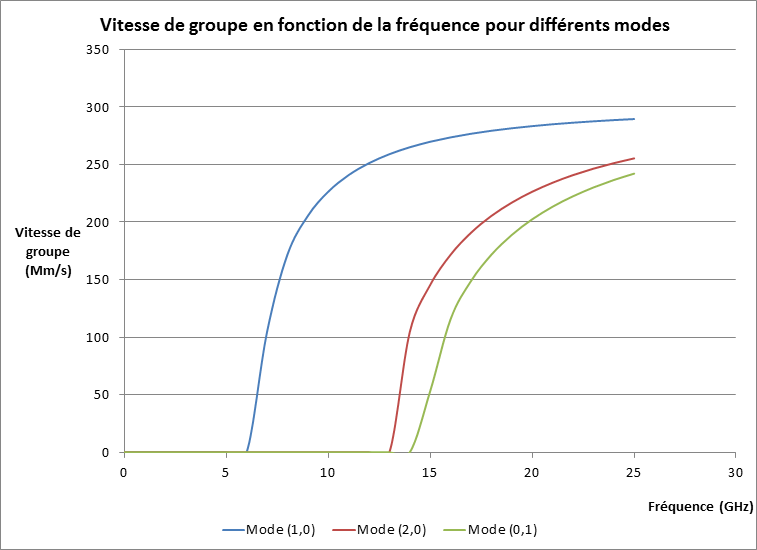
\includegraphics[scale=0.45]{fig2.png}
    \caption{Figure présentant la vitesse de groupe d'une onde en fonction de la fréquence de fonctionnement pour 3 différents modes TE}
    \label{fig1}
\end{figure}

\subsection{Calcul de la longueur d'onde $\lambda_g$ selon la fréquence}
La longueur d'onde dans le guide est donnée par l'équation suivante :

\begin{equation}
	\lambda_g = \frac{\lambda}{\sqrt{1-\left(\frac{f_c}{f}\right)^2}}
\end{equation}
Où:
\begin{itemize}
	\item $\lambda$ est la longueur d'onde du signal traversant le guide; 
	\item $f_c$ est la fréquence de coupure pour un mode donné;
	\item $f$ est la fréquence de l'onde dans le guide.
\end{itemize}


Sachant que la longueur d'onde dans le guide est donnée par l'équation \ref{eq1}, il est possible de trouver $\lambda_g$ pour une fréquence entre 0 et 25 GHz. Les longueurs d'ondes guidées sont affichées à la figure \ref{fig2}. Comme précédemment, les 3 différents modes sont affichés sur la figure et les résultats numériques ne sont pas affichés pour simplifier la présentation du rapport.

\begin{figure}[htbp]
    \centering
    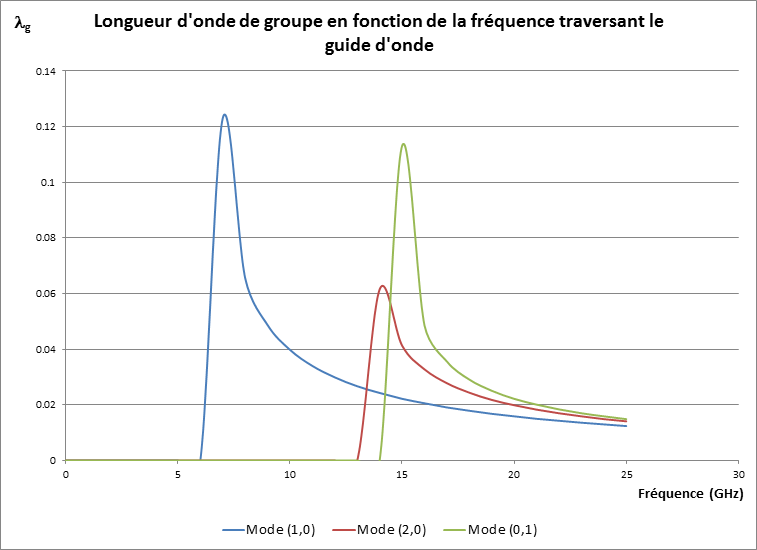
\includegraphics[scale=0.45]{fig1.png}
    \caption{Figure présentant la longueur d'onde guidées en fonction de la fréquence de fonctionnement pour 3 différents modes TE}
    \label{fig2}
\end{figure}

\begin{equation}
	\label{eq1}
	\lambda = \frac{v_p}{f}
\end{equation}

\subsection{Calcul de la l'impédance intrinsèque transverse du guide $\eta_{GTE}$ selon la fréquence}
L'impédance intrinsèque transverse peut être obtenue à l'aide de l'équation suivante :
\begin{equation}
	\eta_{GTE} = \frac{\eta}{\sqrt{1-\left(\frac{f_c}{f}\right)^2}}
\end{equation}
Où:
\begin{itemize}
	\item $\eta$ est l'impédance intrinsèque du guide d'onde, dans notre cas $\eta = 377\Omega$, car nous sommes dans l'air;
	\item $f_c$ est la fréquence de coupure pour un mode donné;
	\item $f$ est la fréquence de l'onde dans le guide.
\end{itemize}

La figure \ref{fig3} représente l'impédance intrinsèque transverse pour les 3 modes d'intérêts entre des fréquences de 0 et 25 GHz.

\begin{figure}[htbp]
    \centering
    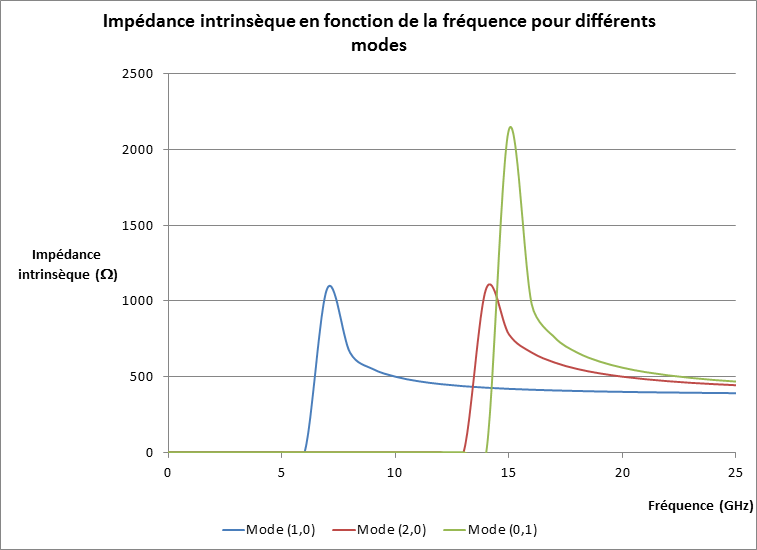
\includegraphics[scale=0.45]{fig3.png}
    \caption{Figure présentant l'impédance intrinsèque d'une guide d'onde en fonction de la fréquence de fonctionnement pour 3 différents modes TE}
    \label{fig3}
\end{figure}


\section{Projet 2: Mesure directe de la fréquence}
Le montage employé pour effectuer les mesures est le montage présenté à la figure \ref{f:fig4}.

\begin{figure}
\centering
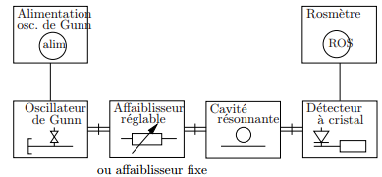
\includegraphics[scale=1]{schema_montage2.png}
\caption{Figure présentant le montage employé lors du projet 2}
\label{f:fig4}
\end{figure}

\paragraph{}Lorsqu'on effectue les mesures avec une tension de 8V, la fréquence à laquelle on note une diminution de l'ordre de 0.5dB à 1.5dB est la fréquence de 10.538GHz. La fraction de la puissance absorbée est de 0.95dB. Comme nous sommes en tension, la fraction de puissance absorbée (\%) correspond à  $100(1- 10^{-0.95/20))\% = 10.36\%$.

\paragraph{}Lorsqu'on effectue les mesures avec une tension de 10V, la fréquence à laquelle on note une diminution de l'ordre de 0.5dB à 1.5dB est la fréquence de 10.541GHz. La fraction de la puissance absorbée est de 0.65dB. Comme nous sommes en tension, la fraction de puissance absorbée (\%) correspond à  $100(1- 10^{-0.65/20))\% = 7.21\%$.

\paragraph{}Lorsqu'on effectue les mesures avec une tension de 4V, le système devient instable et les mesures sortent des plages établies plus tôt. Le système devient très sensible au bruit. L'amplitude de la tension n'est pas contenue dans un seul mode et comme on travaille dans une échelle de puissance très faible (-50dB), l'impact du bruit sur le signal devient très grand à mesure que l'on diminue la tension.

\section{Projet 3: Mesure directe de la fréquence}

\section{Projet 4: Couplage et directivité}
Ce projet est séparé en 2 partie. La première partie consiste à effectuer le montage de la figure \ref{montage1} pour calibré l'entrée du coupleur directif à un niveau relatif de -30 dB sur le ROS-Mètre. Une fois l'atténuateur calibré, il faut effectuer le seconde montage présenté à la figure \ref{montage2} et mesurer le niveau relatif au ROS-Mètre La différence entre ce point de fonctionnement et le point relatif de -30 dB obtenue précédemement donne le couplage du coupleur directif.

\begin{figure}[htbp]
    \centering
    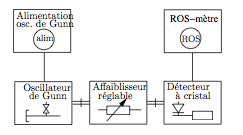
\includegraphics[scale=0.65]{montage1.png}
    \caption{Montage devant être effectué pour calibrer le ROS-Mètre à -30 dB}
    \label{montage1}
\end{figure}

Pour obtenir l'atténuation entre la sortie 3 et la sortie 4, il suffit de procéder de la manière. À partir du montage \ref{montage2}, on calibre le ROS-Mètre à -30 dB à l'aide de l'atténuateur variable. Par la suite, en inversant la charge de la sortie 4 et le détecteur à cristal de la sortie 3, on trouve le niveau relatif de tension pour ce fonctionnement. La différence entre ce point de fonctionnement et le point relatif de -30 dB obtenue précédemement donne la directivité du coupleur.

Dans notre cas, nous trouvons une valeur de couplage de -20.6 dB et une directivité de -26.5 dB.

\begin{figure}[htbp]
    \centering
    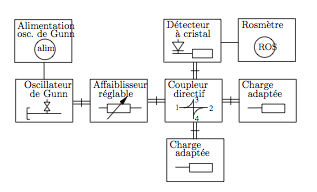
\includegraphics[scale=0.65]{montage2.png}
    \caption{Montage devant être effectué pour mesurer le couplage d'une coupleur directif}
    \label{montage2}
\end{figure}

\section{Projet 5: Impédance caractéristique}

